  \documentclass[10pt]{beamer}
%\documentclass{article}
%\usepackage{beamerarticle}
% for themes, etc.
%{
  %\usetheme{Szeged}
  \usetheme{Warsaw}
  % possiblities Singapore, Malmoe, Dresden
 % \setbeamercovered{transparent}
%}

\setbeamertemplate{navigation symbols}{}
% removes the navigation symbols
%\usecolortheme{crane}

\setbeamercolor*{palette secondary}{use=structure,fg=white,bg=structure.fg!60!blue}
\setbeamercolor*{palette tertiary}{use=structure,fg=white,bg=orange!85!blue}

\def\colorize<#1>{%
 \temporal<#1>{\color{black!20}}{\color{black}}{\color{black!20}}}

%\mode<presentation> { \usetheme{boxes} }

\usepackage{palatino}  % fonts are up to you
\usepackage{graphicx}
\usepackage{amsmath}
\usepackage{amssymb}
\usepackage{epstopdf}
\usepackage{multimedia}
\usepackage[absolute,overlay]{textpos}
\usepackage[document]{ragged2e}

\newenvironment{reference}[2]{                            %
  \begin{textblock*}{\textwidth}(#1,#2)                   % This is the code
      \footnotesize\it\bgroup\color{white}}{\egroup       % for the emulated
  \end{textblock*}}                                       % footnote environment

%\usepackage{media9}

% these will be used later in the title page
%\title{An Operator Splitting Method for Heterogeneous Multiscale Poroelasticity}
%\author{Paul M. Delgado \\ 
%University of Texas at El Paso}
           
%\date{\today}

% note: do NOT include a \maketitle line; also note that this title
% material goes BEFORE the \begin{document}

% have this if you'd like a recurring outline
%\AtBeginSection[]  % "Beamer, do the following at the start of every section"
%{
%\begin{frame}<beamer>
%%\frametitle{Outline} % make a frame titled "Outline"
%\tableofcontents[currentsection]  % show TOC and highlight current section
%\end{frame}
%}
%%%%%%%%%%%%%%%%%%%%%%%%%%%%%%%%%%%%%%%%%%%%%%%%%%%%%%
% Graphs path to the Picture Folder
%%%%%%%%%%%%%%%%%%%%%%%%%%%%%%%%%%%%%%%%%%%%%%%%%%%%%%
%\graphicspath{/home/henry/Desktop/UTEP_Proposal_Thesis/PhD_Thesis/Pictures}
\graphicspath{{Pictures/}{Data/}} % Two folders Picture and Data    
    
\begin{document}
% this prints title, author etc. info from above
%\begin{frame}
%\titlepage
%\end{frame}
\section{The SIAM Computational Methods \& Tools Seminar Proudly Presents:}
\begin{frame}
%\frametitle{An Introduction to \LaTeX}
\frametitle{How to use BLAS and LAPACK with C Programming}

\vskip-0.6cm

\begin{columns}[t]
%%%%%%%%%%%% COLUMN 1  %%%%%%%%%%%%%%%%
	\begin{column}{.3\textwidth}
		%\vspace*{0.2cm}
		%\begin{center} 
		\begin{block}
		\centering
		%\end{center}
		\begin{figure}
			%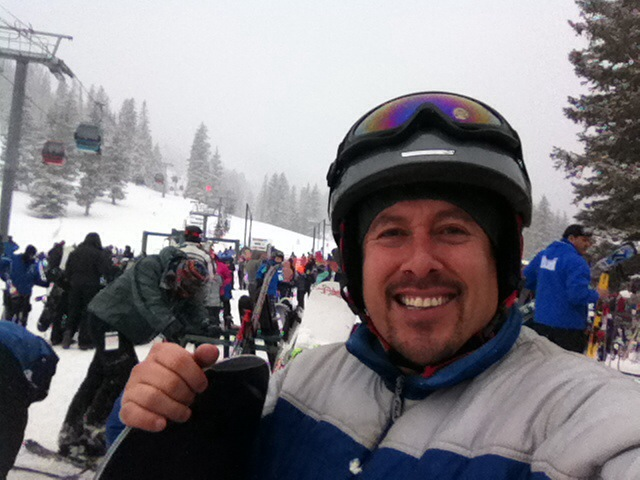
\includegraphics[width=1.3in]{Henry_4.jpg}
			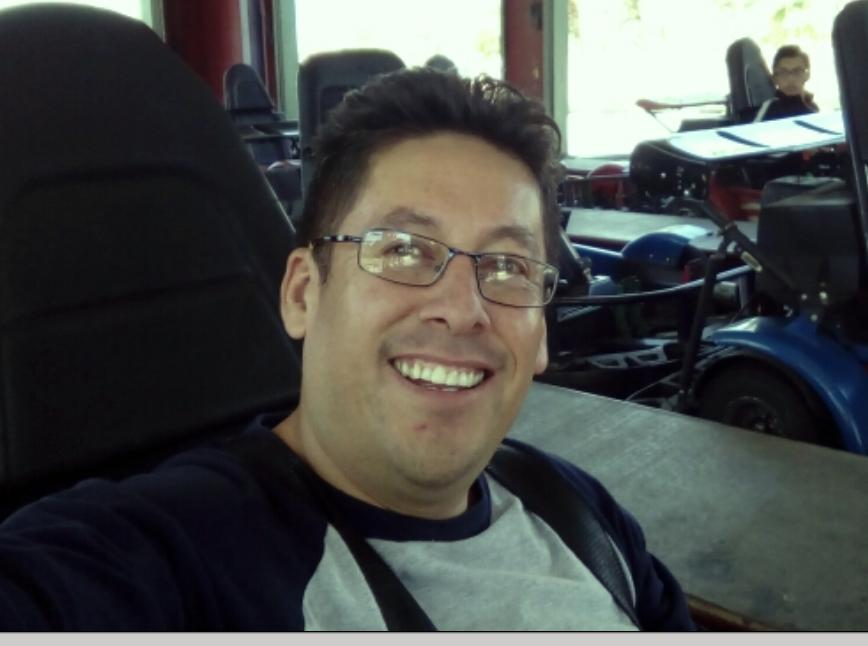
\includegraphics[width=1.3in,height=1in]{Henry.jpeg}
			%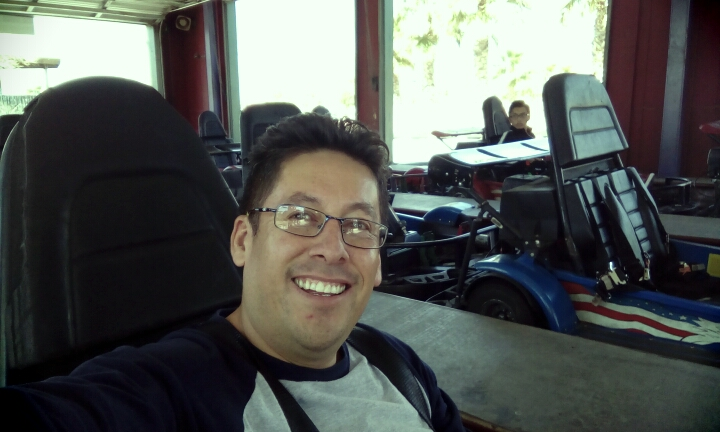
\includegraphics[width=1.3in,height=1in]{IMG_20170319_175240.jpg}
			%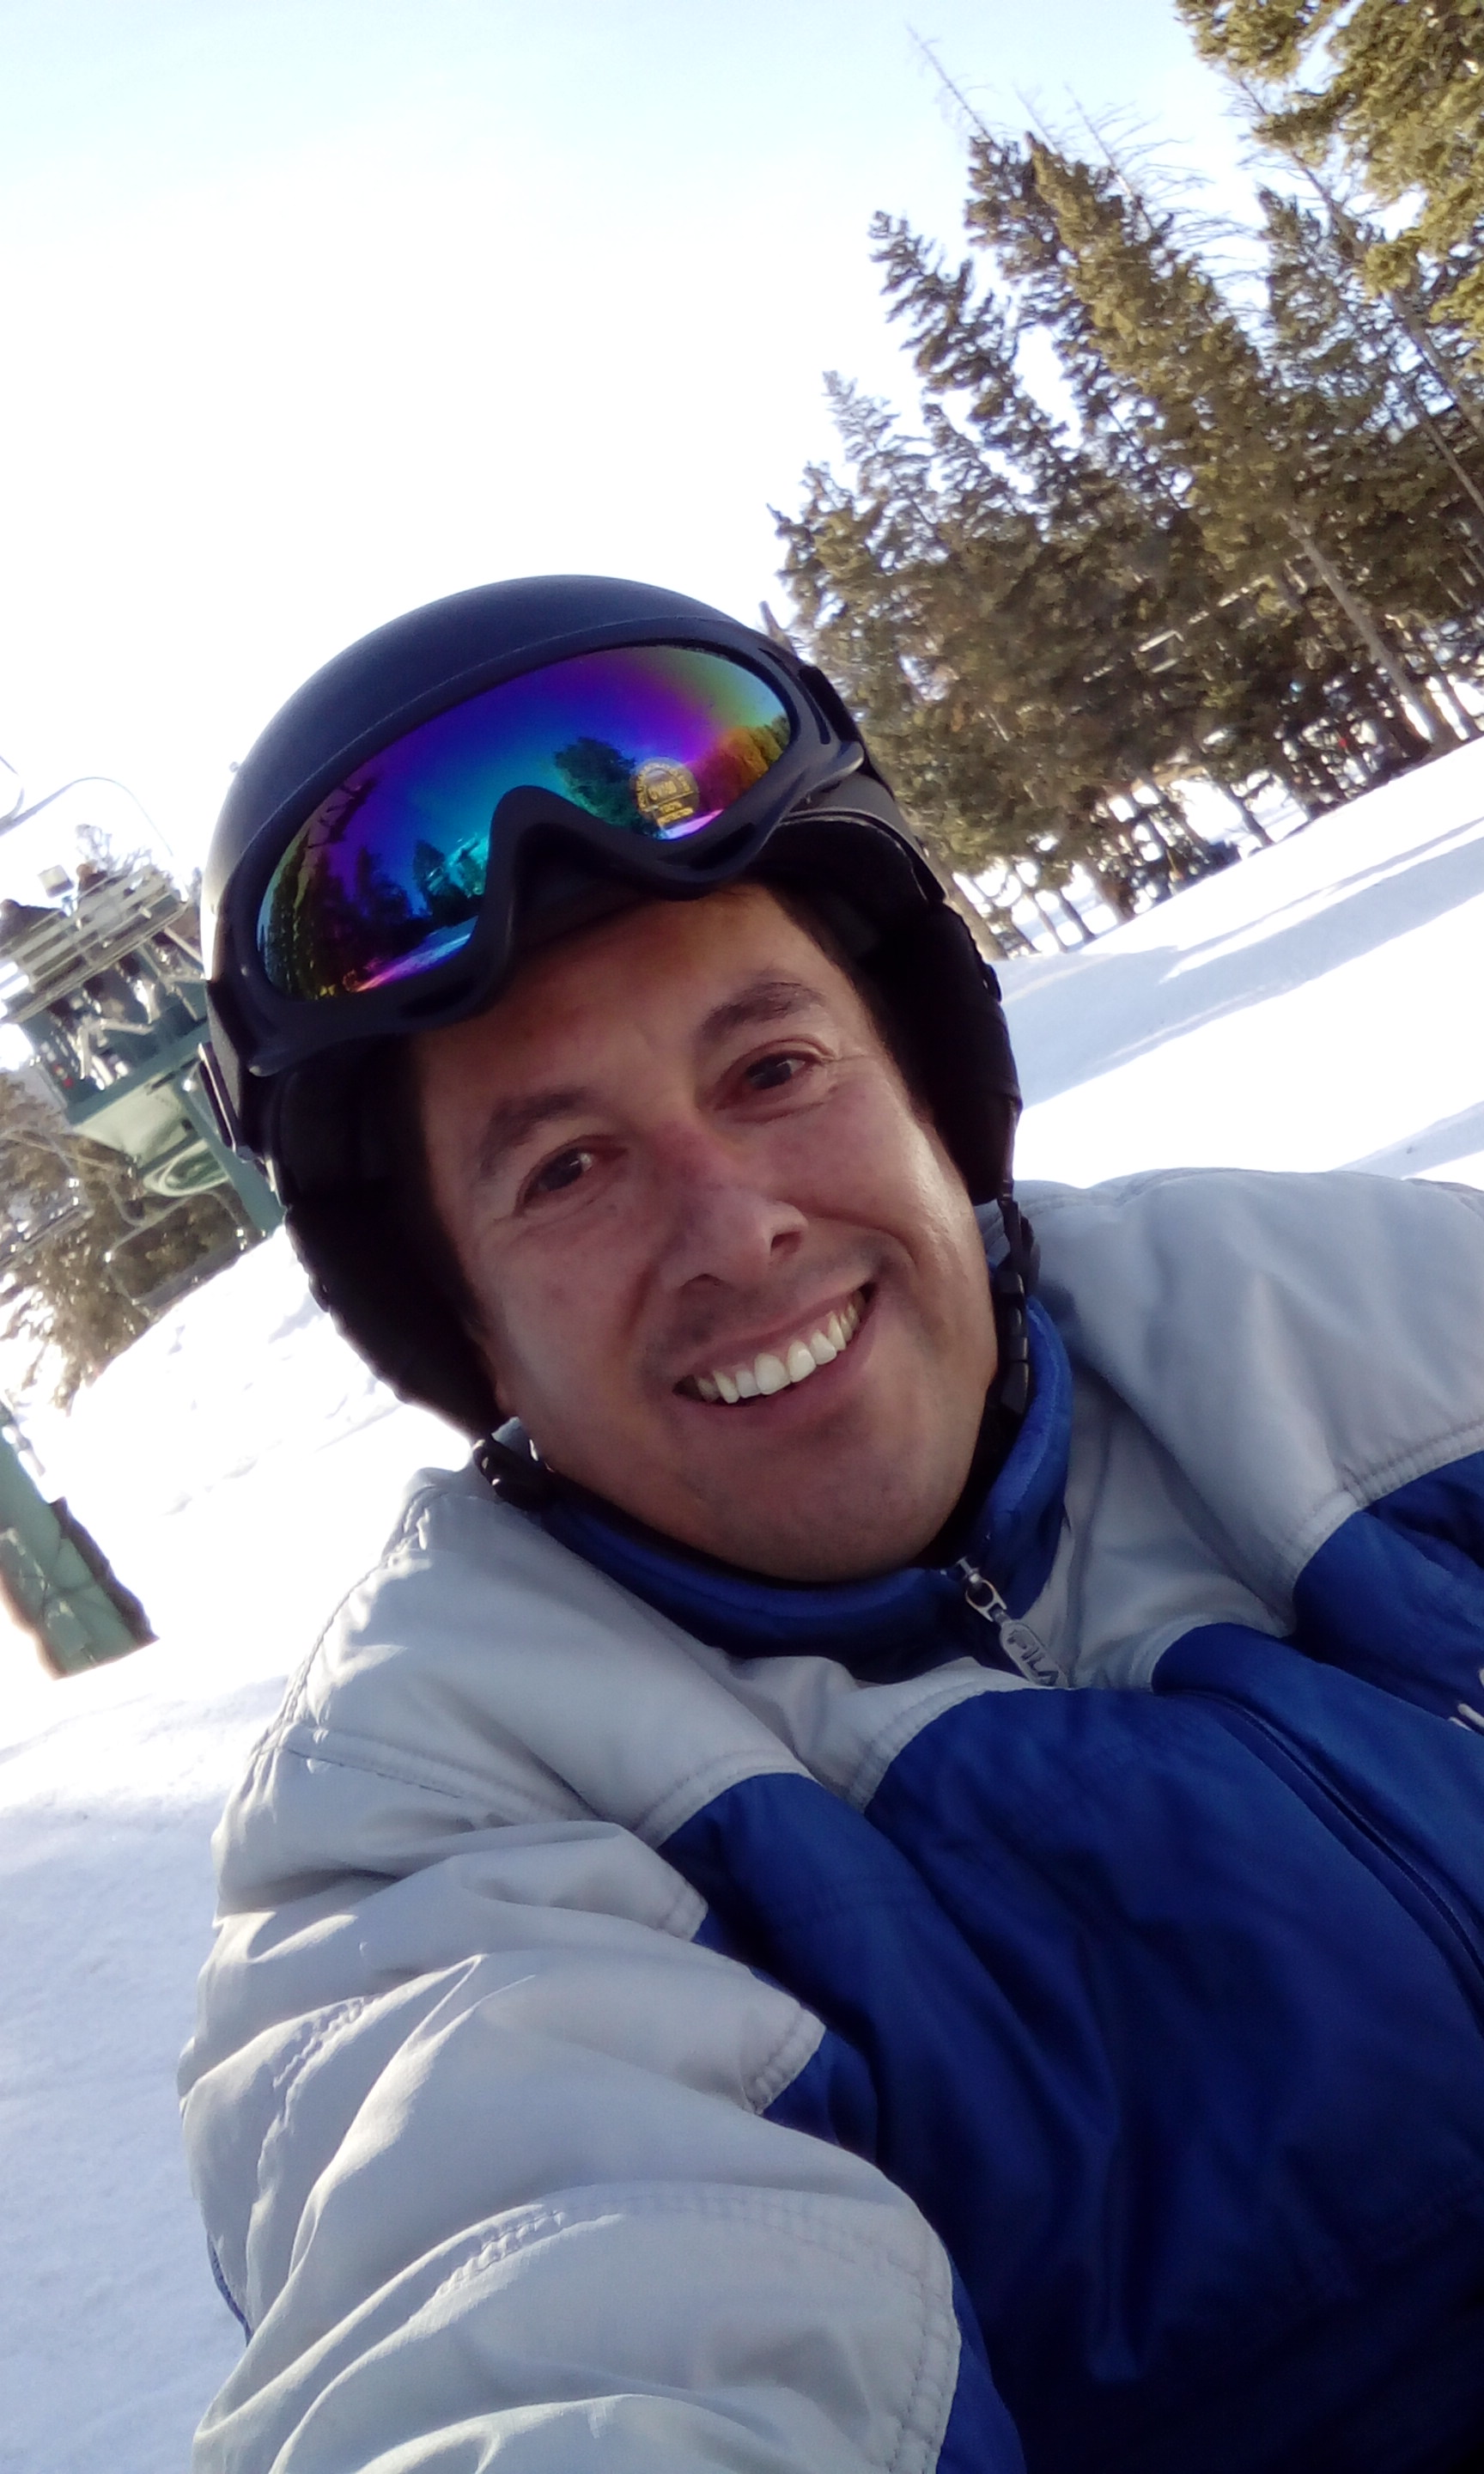
\includegraphics[width=1in,height=1in]{2017_02_11_15_12_26.jpg}
			%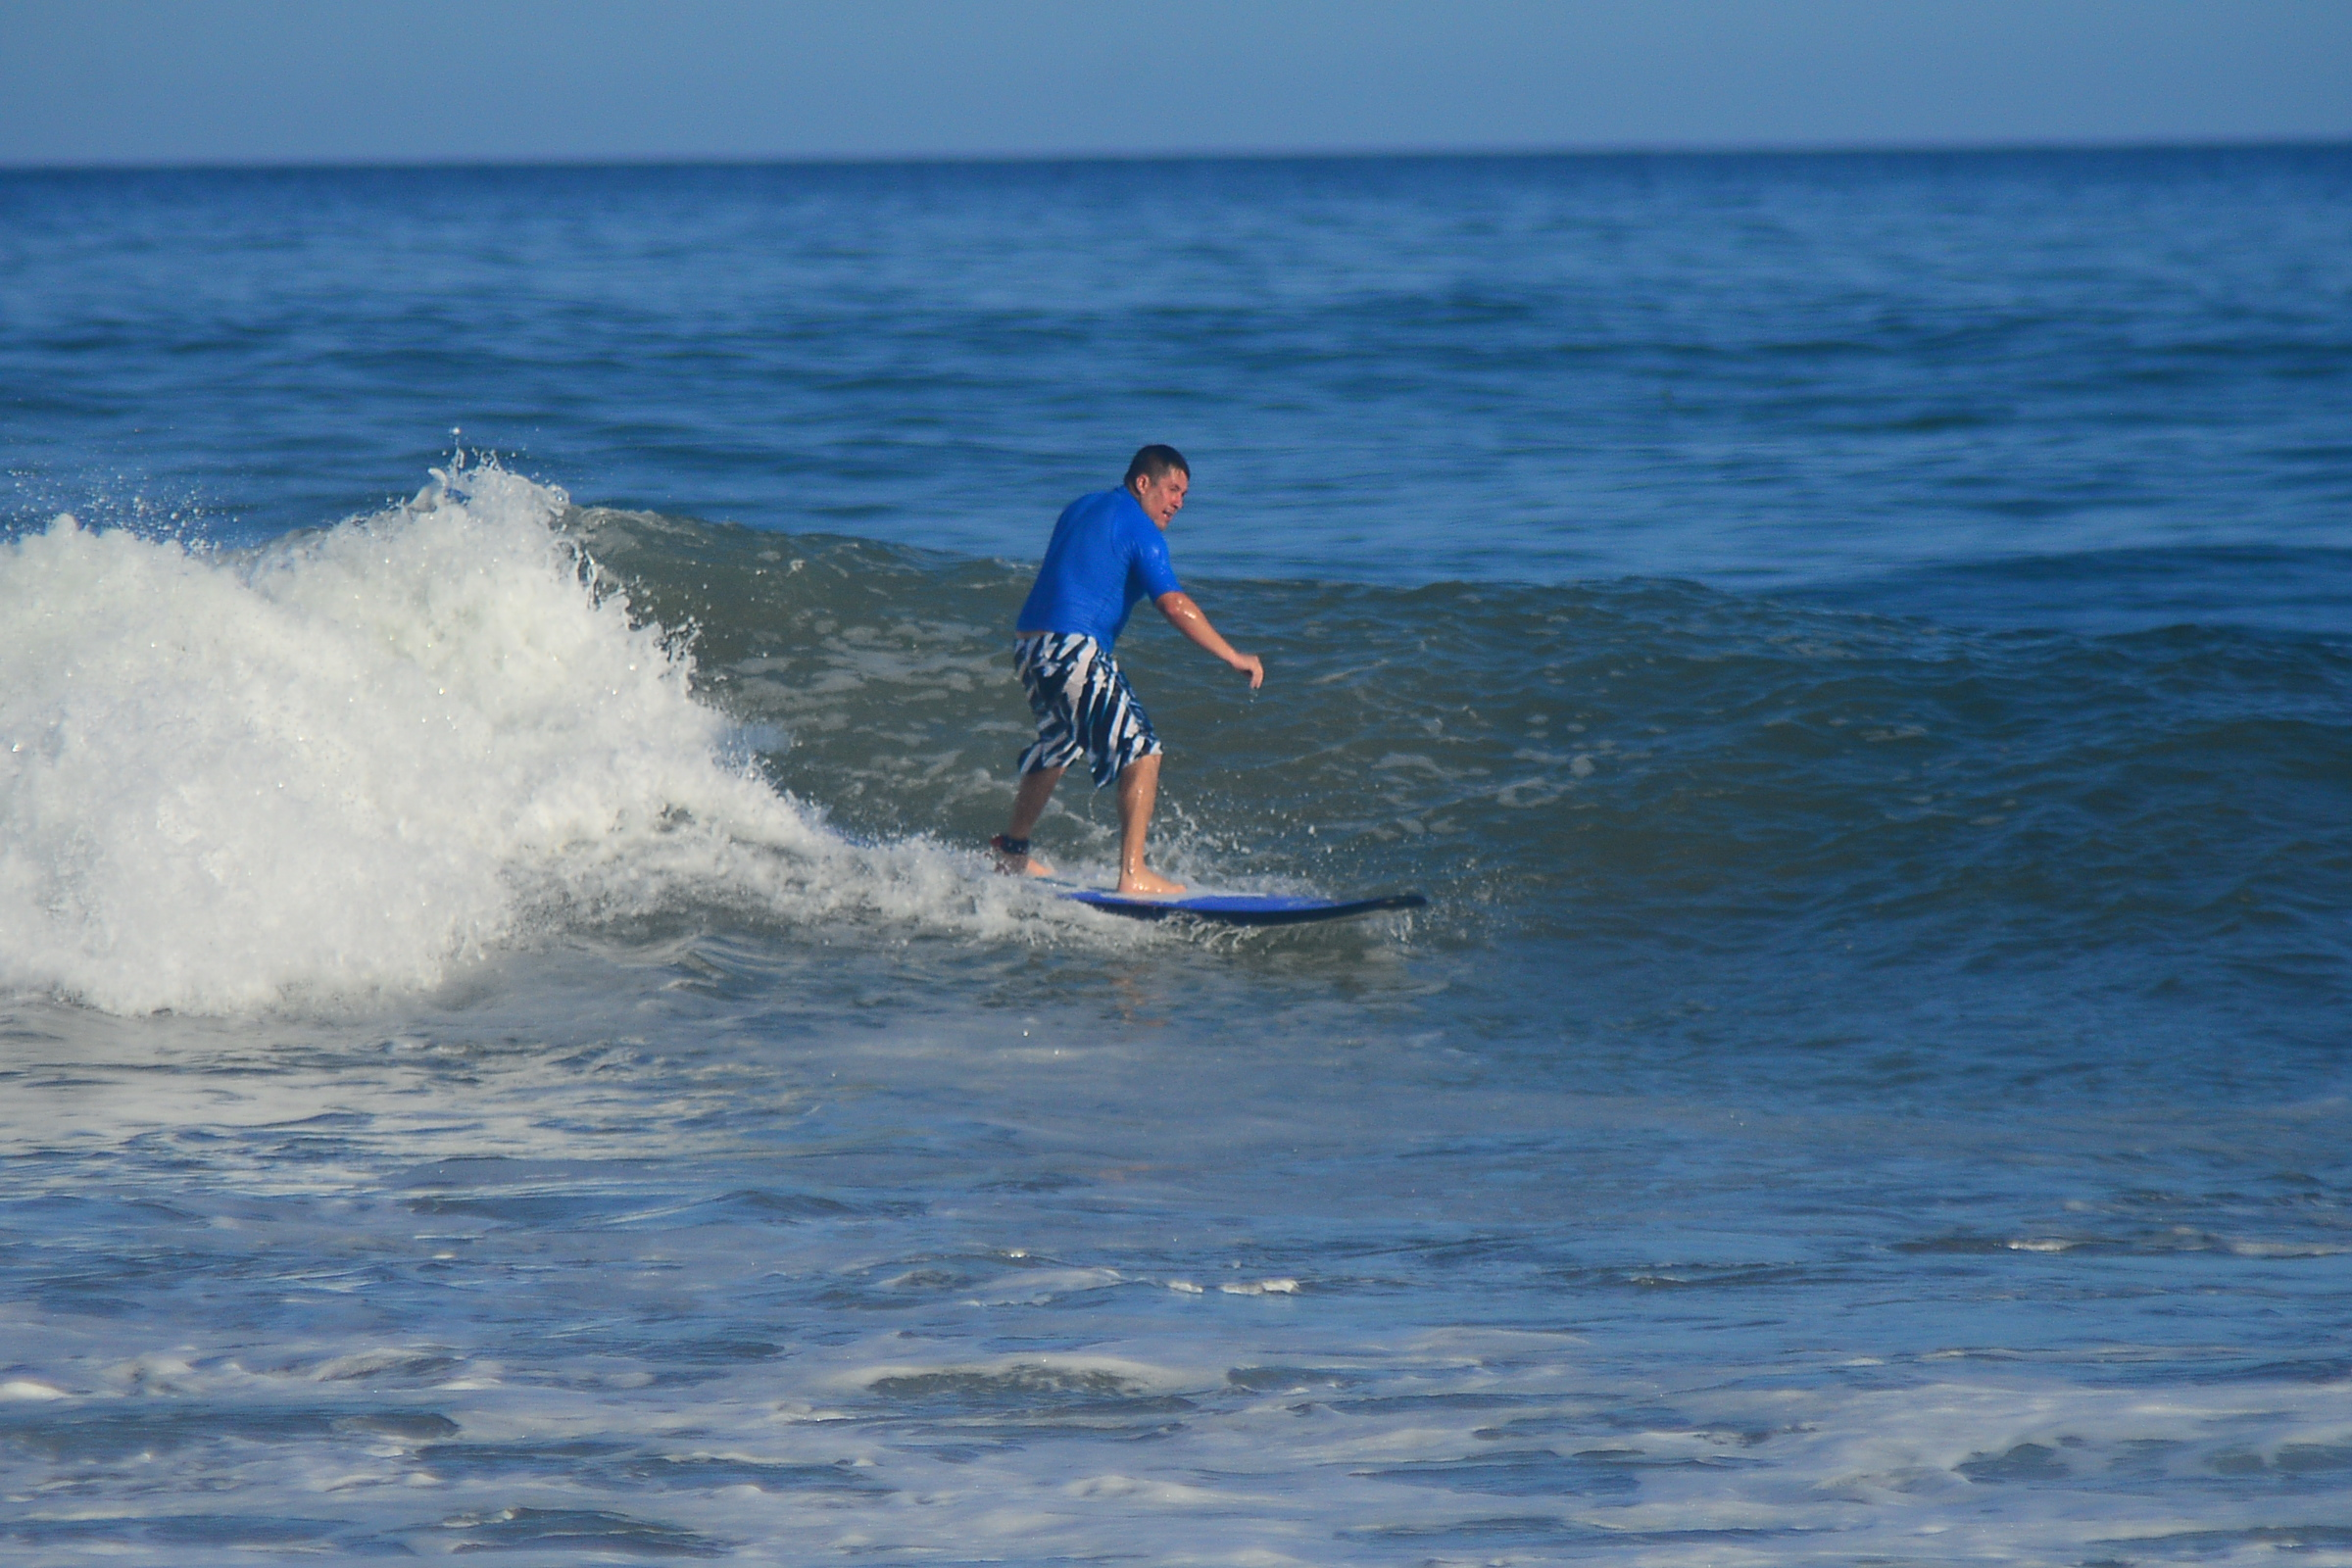
\includegraphics[width=1.2in]{DSC_5706.jpg}
			%\includegraphics[width=1.2in]{2017_02_11_12_01_59.jpg}
			%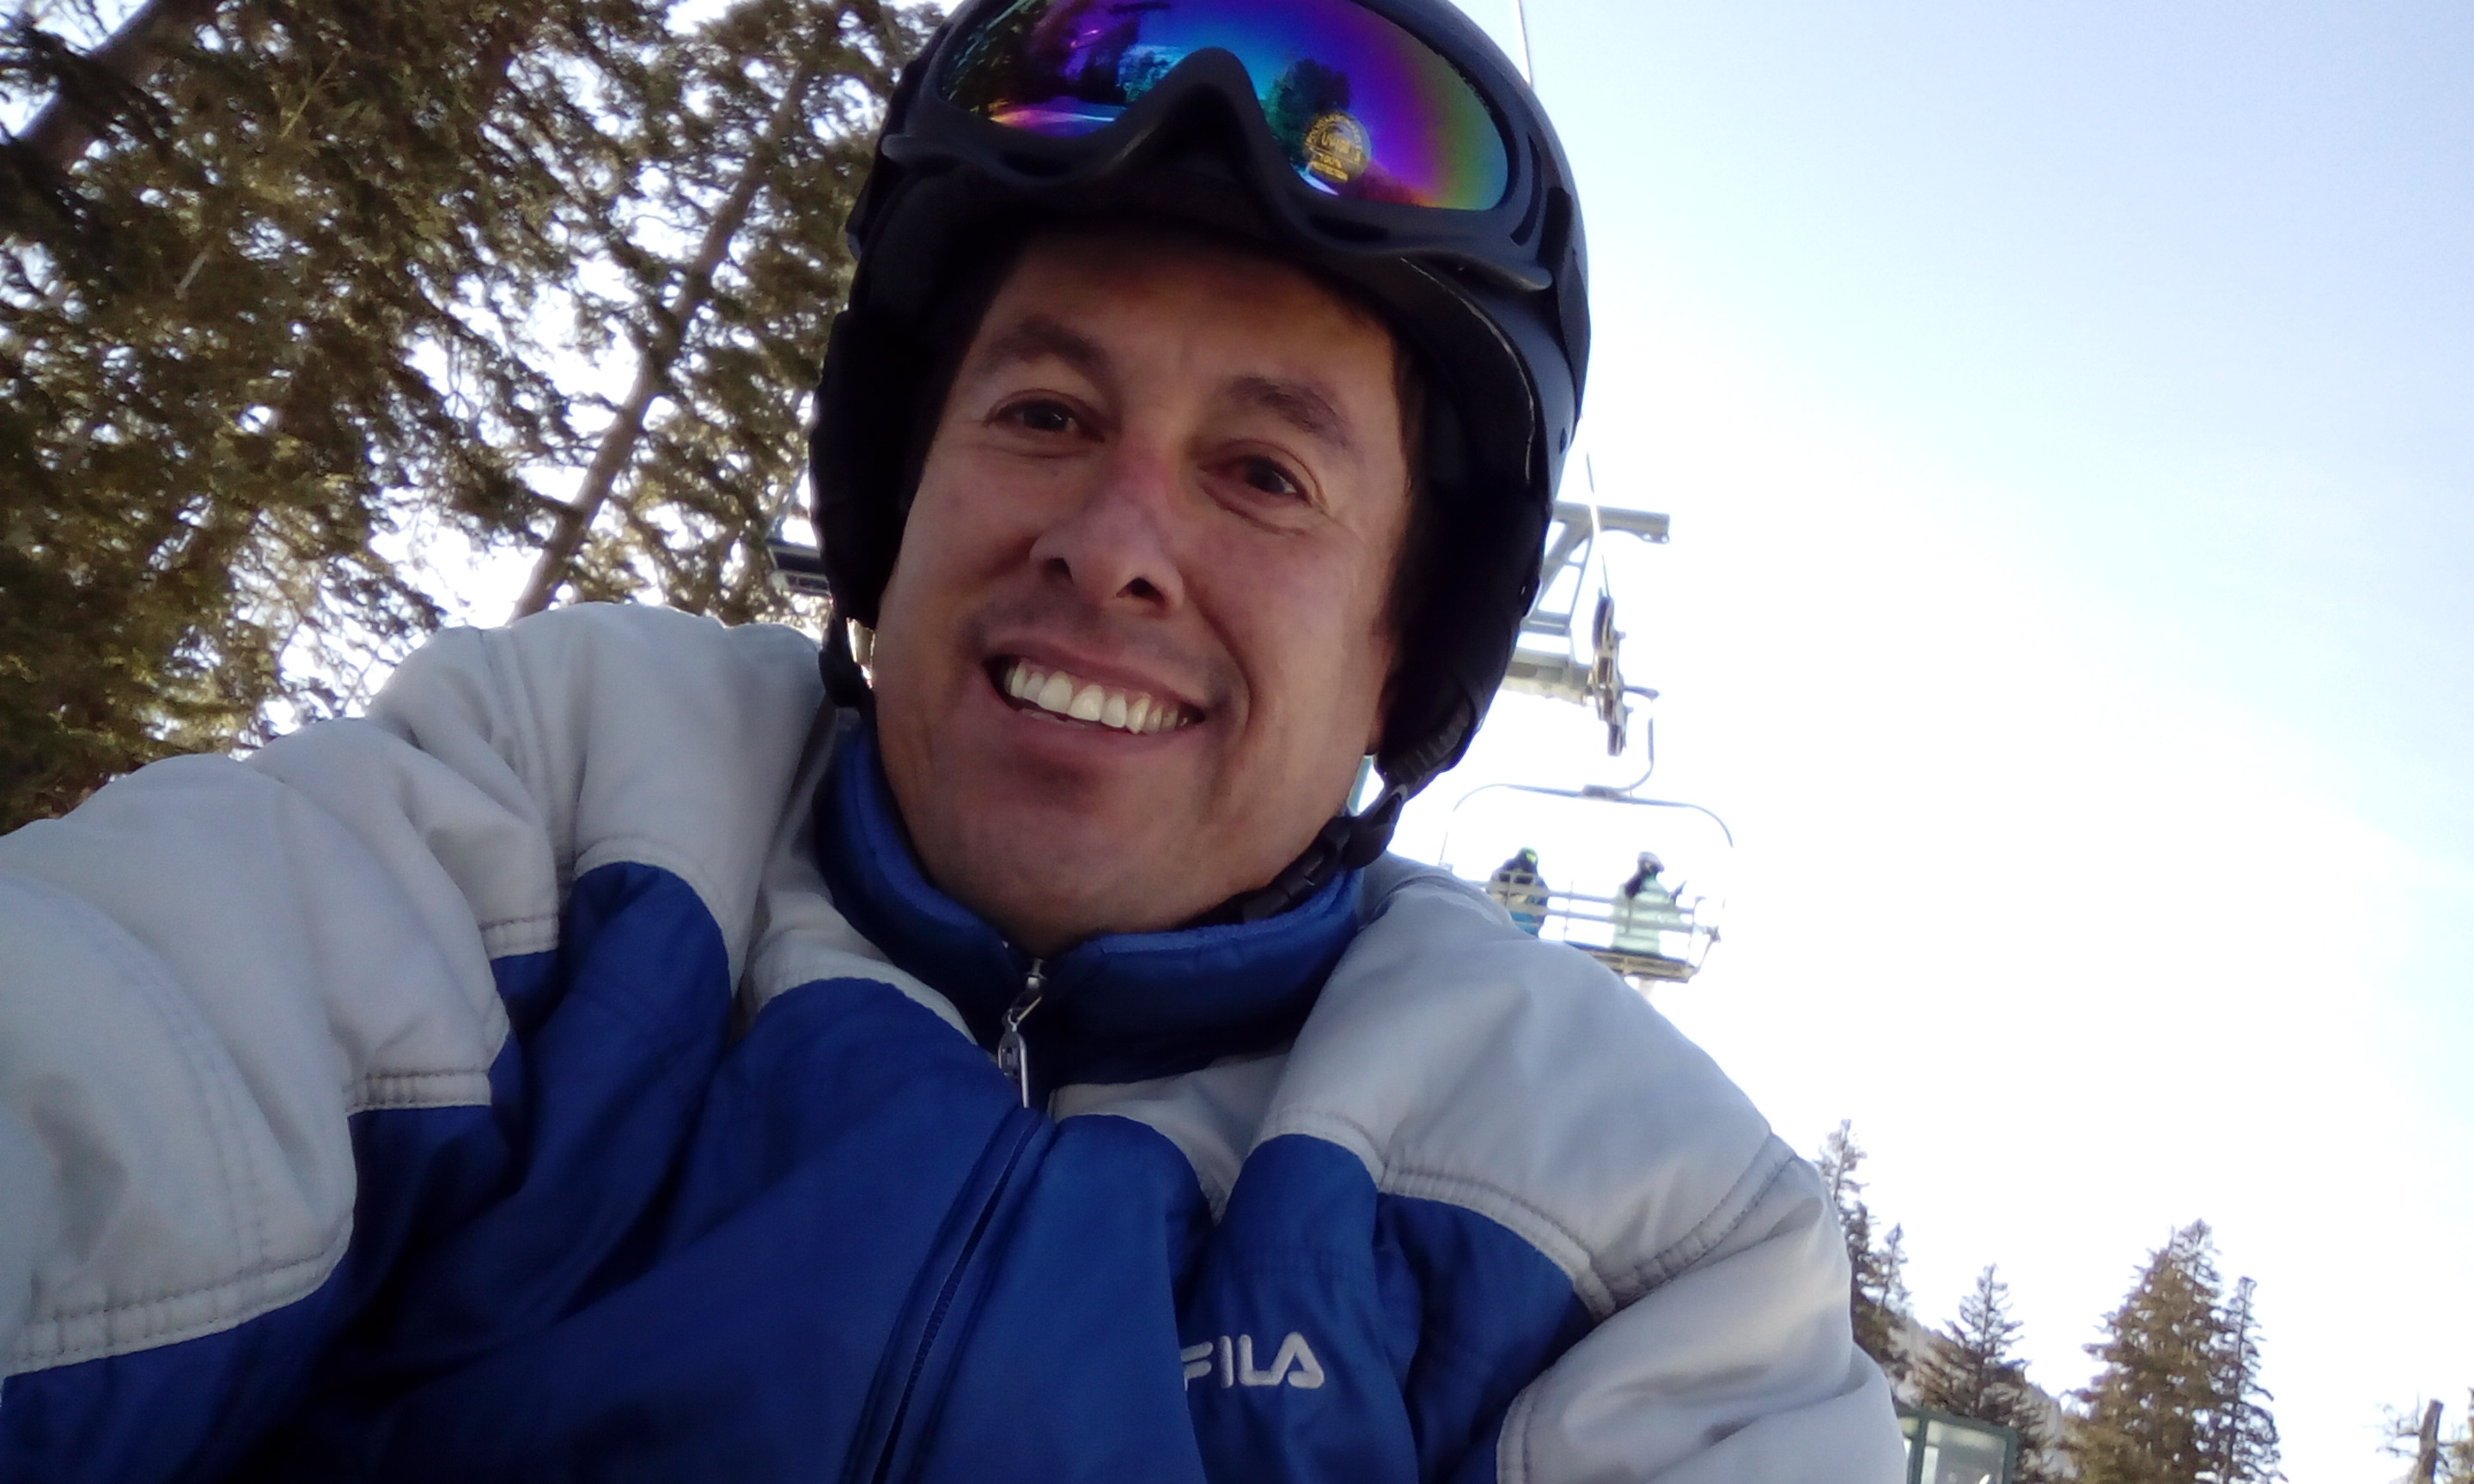
\includegraphics[width=1.2in]{2017_02_11_15_12_36.jpg}
		\end{figure}
%%%%%%%%%%%%%%%%%%%%%%%%%%%%%%%%%%%%%%%%%%%%%%%%%%%%%%%%%%%%%%%%%%%%%%%%%%%%%%%%%%%%%%%%%%%%%%%%%%%%%%%%%%%%%%%%%%%%%
% Install imagemagick :  Using a terminal where the pdf is located:
% 
% >>> convert -density 150 input.pdf -quality 90 output.png

% whereby:
% PNG, JPG or (virtually) any other image format can be chosen
% -density xxx will set the dpi to xxx (common are 150 and 300)
% -quality xxx will set the compression to xxx for PNG, JPG and MIFF file formates (100 means no compression)
% all other options (such as trimming, grayscale, etc) can be viewed on the website of Image Magic.
%%%%%%%%%%%%%%%%%%%%%%%%%%%%%%%%%%%%%%%%%%%%%%%%%%%%%%%%%%%%%%%%%%%%%%%%%%%%%%%%%%%%%%%%%%%%%%%%%%%%%%%%%%%%%%%%%%%%%
		\vskip-0.2cm
		\scriptsize \textbf{Speaker Profile:} \\
		\vskip0.1cm		
		\justifying \tiny \textbf{Henry R. Moncada} is a Ph.D Student in the Computational Science Program at UTEP. He has a BS in Physics from Universidad Nacional Mayor de San Marcos (Peru) and an MS in Applied Mathematics from the University of New Mexico. He was president of UTEP-SIAM Chapter on 2014.
		He was also the recipient of the Good Neighbor Scholarship from 2013 to 2016 and current ASTRO program participant at Oak Ridge National Laboratory (ORNL).
		\end{block} 
	\end{column}
%%%%%%%%%%%% COLUMN 2  %%%%%%%%%%%%%%%%
	\begin{column}{.5\textwidth}
		%\begin{center} 

		%\vspace*{0.5cm}
		
		\justifying \scriptsize \textbf{ABSTRACT:}\\	
		%\vspace*{0.2cm}
	\begin{scriptsize}\textbf{BLAS (Basic Linear Algebra Subprograms)} is a collection of low-level matrix and vector arithmetic operations, for performing common linear algebra operations such as vector addition, scalar multiplication, dot products, linear combinations, and matrix multiplication, and \textbf{LAPACK (Linear Algebra Package)} is a collection of higher-level linear algebra operations that provides routines for solving systems of linear equations such as matrix factorizations (LU, LLt, QR, SVD, Schur, etc), linear least squares, eigenvalue problems, and singular value decomposition. LAPACK is built on top of the BLAS; many users of LAPACK only use the LAPACK interfaces and never need to be aware of the BLAS at all. 
	%LAPACK is generally compiled separately from the BLAS, and can use whatever highly-optimized BLAS implementation you have available. What you should use BLAS and LAPACK depends somewhat on details of what you are trying to do and what platform you are using. 
	In addition, BLAS and LAPACK are incorporated on other computer programs and you used without knowing it. For example, MATLAB uses the Intel Math Kernel Library (MKL) behind the scenes to perform many linear algebra operations.	\end{scriptsize}
		%\vspace*{0.4cm}
		
		\small \textbf{Date:} Friday, April 28th\\
		\vspace*{0.1cm}
		\textbf{Time:} 12:00pm \\
		\vspace*{0.1cm}
		\textbf{Location} CRBL 402.
%		\end{center}
	\end{column}
%%%%%%%%%%%% COLUMN 3  %%%%%%%%%%%%%%%%
	\begin{column}{.2\textwidth}
		\begin{figure}[t!]
		%
\includegraphics[width=.7in]{siam.jpg}
		
\includegraphics[width=.8\textwidth, height=.4\textwidth]{siam.jpg}
		\end{figure}
		\begin{figure}[t!]
		%
\includegraphics[width=.7in]{cps.png}
		
\includegraphics[width=.8\textwidth, height=.4\textwidth]{cps.png}
		\end{figure}
		\begin{figure}[t!]
		%
\includegraphics[width=.7in]{sga.png}
		
\includegraphics[width=.8\textwidth, height=.4\textwidth]{sga.png}
		\end{figure}
	\end{column}
\end{columns}
%\vskip0.5cm
\begin{scriptsize}Free \textbf{snacks} \& \textbf{refreshments} courtesy of the SIAM Student Organization and the UTEP Student Government Association.\end{scriptsize}
  \begin{reference}{5mm}{93mm}                           					% this is the code used inside a                      
  For more details, contact: Henry R. Moncada \hspace*{1.5cm} hrmoncadalopez@miners.utep.edu\\  % frame to state the position    of the footnote
  SIAM PRESIDENT: Griselda Acosta             \hspace*{1.5cm} gvacosta@miners.utep.edu\\
  SIAM VICE PRESIDENT: Bethuel Khamala        \hspace*{1.5cm} bokhamala@miners.utep.edu\\   
  FACULTY ADVISOR: Dr. Natasha Sharma\\
  \end{reference}                                         							
\end{frame}
\end{document}
